\documentclass[10pt, a4paper, twocolumn]{article}
\usepackage[utf8]{inputenc}
\usepackage{graphicx}
\usepackage{geometry}
\usepackage{times}
\usepackage{cite}
\usepackage{amsmath}
\usepackage{amssymb}
\usepackage{booktabs}
\usepackage{multirow}
\usepackage{url}
\usepackage{hyperref}
\usepackage{enumitem}
\usepackage{tikz}
\usetikzlibrary{positioning}
\usepackage{xcolor}
\usepackage{algorithm}
\usepackage{algpseudocode}
\usepackage{caption}
\usepackage{subcaption}

% Workaround for stray control character accidentally introduced during editing
\DeclareUnicodeCharacter{0001}{}

\geometry{top=2cm, bottom=2cm, left=1.5cm, right=1.5cm}
\setlength{\emergencystretch}{3em}
\sloppy
\hfuzz=30pt
\hbadness=10000

\hypersetup{
    colorlinks=true,
    linkcolor=blue,
    citecolor=blue,
    urlcolor=blue
}

\title{\textbf{MANJU: A Multi-Agent Framework for Natural Just-in-Time Understanding in Thai Voice-Based Customer Service}}

\author{
    Sawit Koseeyaumporn, Siratee Saiprom, Sansiri Tarnpradab \\
    \textit{Department of Computer Engineering} \\
    \textit{King Mongkut's University of Technology Thonburi} \\
    \textit{Bangkok, Thailand} \\
    \texttt{\{sawit.kosee, siratee.saip, sansiri.tar\}@kmutt.ac.th}
}

\date{}

\begin{document}

\maketitle

\begin{abstract}
This paper presents \textbf{MANJU} (Multi-Agent AI for Natural Just-in-Time Understanding), an end-to-end automated platform designed to optimize customer service operations through high-availability, real-time Thai voice interaction.
Traditional service channels suffer from personnel shortages and latency during peak hours; MANJU addresses these challenges by integrating Thai Automatic Speech Recognition (ASR), intent-driven multi-agent orchestration, Retrieval-Augmented Generation (RAG), and natural voice synthesis into a unified, low-latency pipeline.
The proposed architecture employs the \textbf{LangGraph} framework to compile user-defined visual workflows into executable state graphs with eight specialized node types---including input, AI reasoning, conditional branching, RAG retrieval, Google Sheets integration, and multimodal output---enabling flexible task decomposition without code changes.
The technical stack incorporates the \textbf{Web Speech API} with Voice Activity Detection (VAD) for real-time speech capture, \textbf{GPT-4o-mini} and \textbf{Qwen3-4B} for language processing, \textbf{FAISS} with \textbf{OpenAI text-embedding-3-small} for semantic retrieval, and \textbf{Qwen3-TTS-12Hz-1.7B} for GPU-accelerated Thai voice synthesis with voice cloning.
The system is implemented as a four-tier microservice architecture (React frontend, Go Fiber API gateway, FastAPI AI orchestrator, and dedicated TTS GPU service) with containerized deployment.
\textbf{Experimental results on a Thai customer-service evaluation set demonstrate sentence-level streaming TTS} achieving a Real-Time Factor (RTF) below 1.0 on NVIDIA G4, and end-to-end response latency within the 5-second target, significantly reducing human workload while maintaining service quality.
\end{abstract}

\vspace{0.5em}
\noindent \textbf{Keywords:} Multi-Agent System, Voice AI, Thai NLP, Retrieval-Augmented Generation, Text-to-Speech, Customer Service Automation, LangGraph.

% ===========================================================================
\section{Introduction}
% ===========================================================================
In the contemporary digital landscape, consumer expectations have shifted toward instantaneous, 24/7 service availability.
Despite this demand, voice-based customer service remains a significant bottleneck: organizational studies indicate that limited human resources and the absence of scalable call center infrastructures lead to delayed responses during peak periods, decreased customer satisfaction, and lost business opportunities~\cite{gans2003callcenters}.

Artificial Intelligence (AI) offers a path toward scalable human-like automation by delegating routine inquiries to AI agents, allowing human staff to focus on high-complexity problems.
However, existing deployed solutions are predominantly text-centric chatbots or rigid Interactive Voice Response (IVR) systems, which lack natural conversational flow, cannot integrate dynamic knowledge sources, and provide no voice cloning or personalization capabilities~\cite{manjuProgReport}.

This study introduces \textbf{MANJU}, a comprehensive end-to-end voice assistant platform tailored for the Thai language.
MANJU bridges the gap between traditional IVR and human-like interaction by combining three core capabilities: (i)~real-time Thai ASR with browser-based VAD, (ii)~LLM reasoning within a user-configurable multi-agent workflow architecture with RAG grounding, and (iii)~high-fidelity Thai TTS with voice cloning via Qwen3-TTS.
Unlike monolithic chatbot designs, MANJU introduces a \textit{workflow-as-data} paradigm: non-technical users visually compose agent graphs in a drag-and-drop editor, and the backend dynamically compiles these into executable LangGraph state machines---enabling domain adaptation without code changes.

\subsection{Objectives}
The objectives of this work are:
\begin{enumerate}[label=(\roman*)]
    \item Develop an end-to-end pipeline spanning speech capture, transcription, multi-agent reasoning with retrieval, and voice synthesis, targeting sub-5-second latency.
    \item Provide a visual workflow editor that enables non-developers to configure agent topologies, knowledge sources, and output modalities.
    \item Implement RAG-grounded responses using FAISS vector search over user-uploaded documents and live Google Sheets data to reduce hallucination.
    \item Evaluate the system on Thai customer-service queries and report latency, routing accuracy, and answer groundedness.
\end{enumerate}

\subsection{Scope}
The current scope covers an MVP supporting FAQ, product information, and knowledge-base inquiries in Thai.
Four workflow modalities are supported: text-to-text, text-to-voice, voice-to-text, and voice-to-voice.
The scope excludes complex multi-turn stateful conversations, emotion analysis, CRM/ticketing integration, and domain-specific model fine-tuning.
The system operates on mixed CPU/GPU resources and supports browser-based voice access~\cite{manjuProgReport}.

\subsection{Contributions}
The contributions of this work are four-fold:
\begin{enumerate}[label=(\roman*)]
    \item \textbf{Workflow-as-Data Architecture:} A visual graph editor that compiles drag-and-drop node configurations into LangGraph \texttt{StateGraph} instances with eight node types and conditional branching.
    \item \textbf{Multi-Agent Orchestration:} LangGraph-based execution supporting intent routing, RAG enrichment, Google Sheets integration, and conditional logic within a single unified state machine.
    \item \textbf{Thai Voice Pipeline:} Integration of Web Speech API with custom VAD for input, and Qwen3-TTS-12Hz-1.7B with sentence-level streaming and voice cloning for output.
    \item \textbf{Production-Grade Platform:} A four-tier microservice deployment with JWT/OAuth authentication, AES-256-GCM encrypted API key management, and Azure Blob/local storage for voice assets.
\end{enumerate}

\noindent\textbf{Paper Organization.}
Section~\ref{sec:related} reviews related work.
Section~\ref{sec:methodology} describes the system architecture and methodology.
Section~\ref{sec:experiments} presents experiments and results.
Section~\ref{sec:conclusion} concludes and outlines future work.

% ===========================================================================
\section{Related Work}
\label{sec:related}
% ===========================================================================

\subsection{Automatic Speech Recognition}
ASR converts speech signals into text using deep learning.
A typical pipeline digitizes audio, extracts acoustic features (e.g., mel-spectrograms), and decodes text via an encoder-decoder or transducer model.
Large-scale end-to-end models such as OpenAI Whisper~\cite{radford2022whisper} demonstrate broad multilingual robustness; however, their non-causal encoder-decoder architecture introduces fundamental limitations for streaming applications: reliance on future context, chunking artifacts that split words, overlapping re-processing overhead, and unpredictable latency from autoregressive decoding.

\subsubsection{Typhoon ASR Real-Time}
Sirichotedumrong et~al.~\cite{sirichotedumrong2026typhoonasr} recently introduced \textbf{Typhoon ASR Real-Time}, a 115M-parameter FastConformer-Transducer model~\cite{rekesh2023fastconformer} specifically engineered for low-latency Thai streaming ASR. The model addresses the critical gap in the Thai ASR landscape, which had been dominated by offline Whisper-based architectures (e.g., Pathumma-Whisper~\cite{tipaksorn2024pathumma}, Thonburian Whisper~\cite{aung2024thonburian}).

Key architectural choices include: (i)~an 8$\times$ depthwise convolutional subsampling encoder that is $\sim$2.4$\times$ faster than standard Conformer~\cite{gulati2020conformer}, (ii)~a Transducer (RNN-T) decoder~\cite{graves2012sequence} enabling true frame-synchronous streaming, and (iii)~a rigorous text normalization pipeline that resolves systemic Thai transcription ambiguities such as context-dependent number verbalization and repetition markers (\textit{mai yamok}).

The model was trained on $\sim$11{,}000 hours of Thai audio curated via a consensus-based pseudo-labeling pipeline using three Whisper-Large teacher models with majority voting. Performance evaluation on the Typhoon ASR Benchmark~\cite{sirichotedumrong2026typhoonasr} demonstrates:
\begin{itemize}[nosep]
    \item \textbf{Competitive accuracy:} CER of 6.81\% on the Gigaspeech2-Typhoon standard track, comparable to the offline Pathumma-Whisper Large-v3 (5.84\% CER) which has 1.55B parameters ($13\times$ larger).
    \item \textbf{Superior robustness:} On the challenging TVSpeech robustness track (in-the-wild Thai media), when trained on the same Whisper Large-v3 architecture, their data pipeline reduces CER from 10.36\% to 6.32\%---a 4.04\% absolute improvement over Pathumma's training data.
    \item \textbf{Extreme throughput:} 4{,}097$\times$ real-time processing speed (RTFx), which is 15--19$\times$ faster than Whisper variants, and $\sim$45$\times$ reduction in computational cost (GFLOPs) compared to Whisper Large-v3.
    \item \textbf{Cost efficiency:} At \$0.0023/hour for 20{,}000 seconds of audio on an NVIDIA L4 GPU---up to 156$\times$ cheaper than the Whisper API and 400$\times$ cheaper than Google/Azure Speech-to-Text.
    \item \textbf{CPU-optimized:} Runs efficiently on standard CPUs without GPU requirements, enabling privacy-first on-premises deployment.
\end{itemize}

\noindent These characteristics make Typhoon ASR Real-Time the ideal candidate for server-side Thai ASR in production voice assistants like MANJU, where low latency, cost efficiency, and on-premises privacy are critical requirements. In MANJU's current MVP, we leverage the browser's Web Speech API (\texttt{webkitSpeechRecognition}) for client-side ASR, augmented with a custom energy-based VAD module; Typhoon ASR is planned as the server-side ASR upgrade for improved domain-specific accuracy (see Section~\ref{sec:conclusion}).

\subsection{Large Language Models}
Transformer-based LLMs~\cite{vaswani2017attention} model long-range token dependencies for contextual understanding and generation.
In customer service, LLMs interpret user intent, generate natural responses, and integrate external knowledge.
GPT-4o-mini~\cite{openai2024gpt4o} provides strong instruction following at reduced cost, while open-weight models like Qwen2.5-7B-Instruct~\cite{qwen2024qwen25} enable deployment on private infrastructure.
MANJU supports configurable LLM selection per workflow node, with provider abstraction via LiteLLM.

\subsection{Text-to-Speech Synthesis}
Modern end-to-end TTS predicts acoustic features and synthesizes waveforms via neural vocoders~\cite{tan2021ttssurvey}.
For Thai, F5-TTS variants support real-time synthesis and voice cloning.
Qwen3-TTS-12Hz-1.7B offers three model variants (base voice cloning, custom preset voices, and text-described voice design), enabling diverse voice personalization with 1.7B parameters and Flash Attention 2 optimization.

\subsection{Multi-Agent LLM Architectures}
Multi-agent architectures decompose reasoning into specialized agents that coordinate via message passing.
AutoGen~\cite{wu2023autogen} demonstrates multi-agent LLM collaboration patterns, while LangGraph~\cite{langgraph2024} provides a graph-based framework for stateful, cyclical agent workflows.
Compared with monolithic designs, explicit agent routing reduces misinterpretation by delegating subtasks (e.g., general conversation vs.\ product lookup vs.\ policy retrieval) to domain-specialized nodes.

\subsection{Retrieval-Augmented Generation}
RAG~\cite{lewis2020rag} combines dense passage retrieval with LLM generation, grounding answers in external sources to reduce hallucination.
FAISS~\cite{johnson2019faiss} provides billion-scale similarity search over dense vectors.
In MANJU, user-uploaded documents (PDF, DOCX, TXT) are chunked, embedded via OpenAI \texttt{text-embedding-3-small}, and indexed in FAISS for per-query retrieval.

\subsection{Voice-Based Customer Service Systems}
Traditional IVR systems provide menu-based automation but lack conversational flexibility~\cite{gans2003callcenters}.
Recent voice assistants combine ASR, LLM-based intent handling, and TTS for more natural dialog, but must address latency constraints and answer groundedness.
MANJU extends this line of work by providing a configurable multi-agent workflow platform with RAG grounding and high-fidelity Thai voice cloning.

% ===========================================================================
\section{Methodology}
\label{sec:methodology}
% ===========================================================================

\subsection{System Architecture Overview}

MANJU is implemented as a four-tier microservice platform, illustrated in Figure~\ref{fig:architecture}.
Each tier can be independently scaled and deployed as a Docker container.

\begin{figure}[t]
    \centering
    \small
    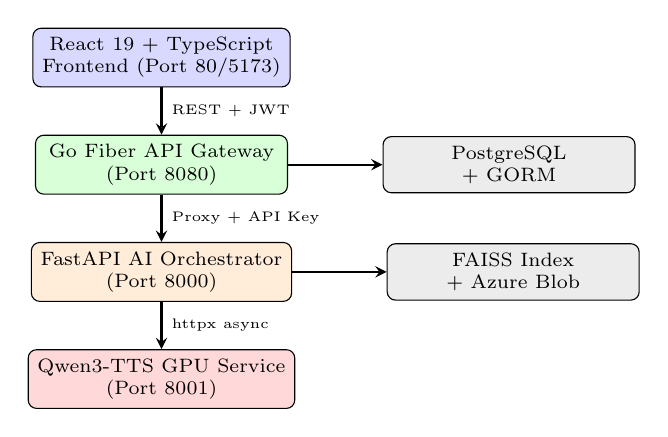
\begin{tikzpicture}[
        node distance=0.6cm,
        box/.style={rectangle, draw, rounded corners=3pt, minimum width=3.2cm, minimum height=0.7cm, align=center, font=\scriptsize},
        arrow/.style={->, thick, >=stealth}
    ]
        % Tier 1: Frontend
        \node[box, fill=blue!15] (frontend) {React 19 + TypeScript\\Frontend (Port 80/5173)};
        
        % Tier 2: Go Backend
        \node[box, fill=green!15, below=of frontend] (gobackend) {Go Fiber API Gateway\\(Port 8080)};
        
        % Tier 3: AI Backend
        \node[box, fill=orange!15, below=of gobackend] (aibackend) {FastAPI AI Orchestrator\\(Port 8000)};
        
        % Tier 4: TTS
        \node[box, fill=red!15, below=of aibackend] (tts) {Qwen3-TTS GPU Service\\(Port 8001)};
        
        % Database
        \node[box, fill=gray!15, right=1.2cm of gobackend] (db) {PostgreSQL\\+ GORM};
        
        % Storage
        \node[box, fill=gray!15, right=1.2cm of aibackend] (storage) {FAISS Index\\+ Azure Blob};
        
        % Arrows
        \draw[arrow] (frontend) -- node[right, font=\tiny] {REST + JWT} (gobackend);
        \draw[arrow] (gobackend) -- node[right, font=\tiny] {Proxy + API Key} (aibackend);
        \draw[arrow] (aibackend) -- node[right, font=\tiny] {httpx async} (tts);
        \draw[arrow] (gobackend) -- (db);
        \draw[arrow] (aibackend) -- (storage);
    \end{tikzpicture}
    \caption{MANJU four-tier microservice architecture. The Go API gateway handles authentication and proxies requests to the FastAPI orchestrator, which compiles workflows and dispatches TTS to a dedicated GPU service.}
    \label{fig:architecture}
\end{figure}

\noindent\textbf{Tier~1: Frontend.}
A React~19 / TypeScript~5.9 single-page application built with Vite~7.2 provides the user interface, including a visual drag-and-drop workflow editor, a demo chat console with voice I/O, voice management, and API key settings.
The frontend uses the Web Speech API for ASR and implements a custom energy-based VAD for automatic silence detection.

\noindent\textbf{Tier~2: API Gateway.}
A Go Fiber HTTP server provides REST API endpoints, Google OAuth~2.0 authentication with JWT (HS256, 7-day expiry), AES-256-GCM encrypted API key storage via GORM/PostgreSQL, and authenticated proxying to the AI services.
It resolves user-provided API keys, loads workflow configurations from the database, injects user/project metadata into RAG nodes, and forwards requests to the AI backend.

\noindent\textbf{Tier~3: AI Orchestrator.}
A FastAPI (Python) service hosts the \texttt{WorkflowExecutor}, which compiles workflow JSON into LangGraph \texttt{StateGraph} instances, executes multi-agent reasoning, performs RAG retrieval via FAISS, and integrates Google Sheets data.

\noindent\textbf{Tier~4: TTS Service.}
A dedicated GPU-accelerated FastAPI service running Qwen3-TTS-12Hz-1.7B models with Flash Attention~2 on NVIDIA H100 GPUs.
Supports three model variants for voice cloning, preset voices, and voice design.

\subsection{ASR Module with Voice Activity Detection}

The ASR module operates entirely in the browser using the Web Speech API (\texttt{webkitSpeechRecognition}) configured for continuous Thai recognition (\texttt{lang=th-TH}) with interim results.
To enable hands-free operation, we implement a custom VAD module using the Web Audio API's \texttt{AnalyserNode}:

\begin{enumerate}[label=\arabic*.]
    \item The microphone stream is connected to an \texttt{AnalyserNode} that computes the RMS energy of each audio frame.
    \item A configurable energy threshold ($\theta_\text{VAD} = 0.01$) distinguishes speech from silence.
    \item When speech energy drops below $\theta_\text{VAD}$ for a silence duration $\tau_\text{silence} = 1100$\,ms, the system automatically submits the accumulated transcript.
    \item The VAD loop runs via \texttt{requestAnimationFrame} for smooth, non-blocking monitoring.
\end{enumerate}

\noindent This approach provides zero-click voice interaction without requiring a push-to-talk button.

\subsubsection{Rationale for Typhoon ASR as Server-Side Upgrade}
While the Web Speech API provides convenient zero-setup ASR via the browser, it has inherent limitations: dependence on the browser vendor's cloud transcription service, limited control over the recognition model, and reduced accuracy on domain-specific Thai terminology. For production deployments requiring privacy, reliability, and domain adaptation, we identify \textbf{Typhoon ASR Real-Time}~\cite{sirichotedumrong2026typhoonasr} as the optimal server-side replacement.

Table~\ref{tab:asr_comparison} summarizes the key comparison. Typhoon ASR's 115M-parameter FastConformer-Transducer achieves CER within 1\% of the 1.55B-parameter Pathumma-Whisper Large-v3 while being 45$\times$ more computationally efficient and supporting true streaming inference. Its CPU-optimized design eliminates GPU costs for ASR, and the open-source MIT license enables full on-premises deployment---a critical requirement for organizations handling sensitive voice data.

\begin{table}[t]
    \centering
    \caption{Comparison of Thai ASR models relevant to MANJU deployment. CER is reported on the Gigaspeech2-Typhoon standard track~\cite{sirichotedumrong2026typhoonasr}. RTFx = real-time factor (higher is faster).}
    \label{tab:asr_comparison}
    \small
    \begin{tabular}{@{}lcccr@{}}
        \toprule
        \textbf{Model} & \textbf{Params} & \textbf{CER} & \textbf{RTFx} & \textbf{Stream} \\
        \midrule
        Pathumma-Whisper Lg-v3 & 1.55B & 5.84\% & $\sim$215 & No \\
        Biodatlab Distil-Whisper & 756M & 8.24\% & $\sim$640 & No \\
        \textbf{Typhoon ASR Real-Time} & \textbf{115M} & \textbf{6.81\%} & \textbf{4{,}097} & \textbf{Yes} \\
        \bottomrule
    \end{tabular}
\end{table}

\noindent Furthermore, Typhoon ASR's compact 115M-parameter model supports fine-tuning on domain-specific vocabulary with minimal resources (even on Google Colab), enabling organizations to adapt recognition for their product names, policies, and jargon---directly improving downstream multi-agent accuracy.

\subsection{Multi-Agent Orchestration via LangGraph}
\label{sec:orchestration}

The core innovation of MANJU is its \textit{workflow-as-data} paradigm: agent topologies are defined as JSON graph structures (nodes and connections) created visually in the frontend, persisted in PostgreSQL, and compiled at runtime into executable LangGraph state machines.

\subsubsection{State Definition}
The workflow operates on a typed state dictionary (\texttt{WorkflowState}) threading through all nodes:

\begin{small}
\begin{verbatim}
WorkflowState = {
  user_message: str,
  conversation_history: List[Dict],
  rag_context: Optional[str],
  sheets_data: Optional[str],
  condition_results: Dict[str, bool],
  output_variables: Dict[str, str],
  response: str,
  nodes_executed: List[str],
  model_used: Optional[str],
  openai_api_key: Optional[str]
}
\end{verbatim}
\end{small}

\subsubsection{Node Types}
The system supports eight node types organized into four categories, summarized in Table~\ref{tab:node_types}.

\begin{table}[t]
    \centering
    \caption{MANJU workflow node types and their functions.}
    \label{tab:node_types}
    \small
    \begin{tabular}{@{}llp{3.8cm}@{}}
        \toprule
        \textbf{Category} & \textbf{Node Type} & \textbf{Description} \\
        \midrule
        \multirow{2}{*}{Input} & \texttt{text-input} & Captures user text message \\
        & \texttt{voice-input} & Voice input via Web Speech API \\
        \midrule
        \multirow{2}{*}{Processing} & \texttt{ai-model} & LLM inference (GPT-4o-mini, Qwen2.5-7B, etc.) with configurable system prompt, temperature, and output variables \\
        & \texttt{if-condition} & Conditional branching with operators: \textit{contains}, \textit{equals}, \textit{regex}, \textit{isYes}, \textit{isNo} \\
        \midrule
        \multirow{2}{*}{Data} & \texttt{rag-documents} & FAISS vector retrieval over uploaded documents \\
        & \texttt{google-sheets} & Live data fetch via \texttt{gspread} \\
        \midrule
        \multirow{2}{*}{Output} & \texttt{text-output} & Returns text response \\
        & \texttt{voice-output} & TTS synthesis (OpenAI or Qwen3) \\
        \bottomrule
    \end{tabular}
\end{table}

\subsubsection{Graph Compilation}
The \texttt{WorkflowExecutor.\_build\_graph()} method converts frontend JSON into a LangGraph \texttt{StateGraph} through the following steps:

\begin{enumerate}[label=\arabic*.]
    \item \textbf{Adjacency construction:} Parse the connections array to build adjacency lists with port information (source/target ports enable conditional routing).
    \item \textbf{Node registration:} For each workflow node, register a corresponding processing function in the \texttt{StateGraph}. Each function reads from and writes to the shared \texttt{WorkflowState}.
    \item \textbf{Edge wiring:} For \texttt{if-condition} nodes, use LangGraph's \texttt{add\_conditional\_edges()} with true/false port routing. For linear nodes, add standard edges.
    \item \textbf{Entry point detection:} The algorithm prefers input nodes as entry points; falls back to RAG or Google Sheets nodes if no explicit input is found.
    \item \textbf{Compilation:} The graph is compiled into an executable instance via \texttt{graph.compile()}.
\end{enumerate}

\noindent Context injection ensures linear execution ordering: when a RAG or Google Sheets node feeds into an AI model, the graph enforces sequential execution (\texttt{input} $\rightarrow$ \texttt{RAG} $\rightarrow$ \texttt{AI model}) rather than parallel branches writing to the same state key.

\subsubsection{Workflow Type Detection}
At request time, the system automatically detects one of four workflow modalities---\textit{text-to-text}, \textit{text-to-voice}, \textit{voice-to-text}, \textit{voice-to-voice}---by scanning node types and determines the TTS provider (\texttt{openai} or \texttt{qwen3}) from voice-output node configuration.

\subsection{Retrieval-Augmented Generation Module}
\label{sec:rag}

The RAG module grounds LLM responses in user-provided documents, following the pipeline:

\begin{enumerate}[label=\arabic*.]
    \item \textbf{Document ingestion:} Users upload PDF, DOCX, or TXT files through the web interface. The Go backend stores files at \texttt{uploads/documents/\{userId\}/\{projectId\}/} and triggers embedding via the AI backend's \texttt{/embed-documents} endpoint.
    \item \textbf{Chunking:} Documents are split using LangChain's \texttt{RecursiveCharacterTextSplitter} with a chunk size of 1{,}000 characters and overlap of 200 characters.
    \item \textbf{Embedding:} Chunks are embedded using OpenAI's \texttt{text-embedding-3-small} model (1{,}536 dimensions).
    \item \textbf{Indexing:} Embeddings are stored in a FAISS flat index, persisted at \texttt{faiss\_indexes/\{userId\}/\{projectId\}/}.
    \item \textbf{Retrieval:} At query time, the user message is embedded and the top-$k$ ($k{=}3$ by default) most similar chunks are retrieved via \texttt{similarity\_search\_with\_score()}.
    \item \textbf{Context injection:} Retrieved passages with source attribution and similarity scores are prepended to the user message before LLM inference.
\end{enumerate}

\noindent The index resolution strategy tries multiple candidate paths in order: (1)~\texttt{userId/projectId}, (2)~\texttt{projectId} only, (3)~\texttt{default}---ensuring backward compatibility across deployment configurations.

\subsection{Google Sheets Integration}

For organizations maintaining dynamic data in spreadsheets, the \texttt{google-sheets} node fetches live data via \texttt{gspread}~6.1.2 with OAuth2 service account authentication.
Data is retrieved as a Pandas DataFrame, converted to a Markdown table (limited to 50 rows to control token budget), and injected into the AI model's prompt as \texttt{sheets\_data}.
This enables real-time access to frequently updated information (e.g., inventory, pricing, schedules) without re-embedding.

\subsection{TTS Module: Dual-Provider Architecture}
\label{sec:tts}

MANJU implements a dual-TTS architecture driven by the \texttt{voice-output} node's \texttt{ttsProvider} field, supporting both cloud and on-premise synthesis.

\subsubsection{OpenAI TTS Path}
For rapid prototyping, the system supports OpenAI's \texttt{tts-1} and \texttt{tts-1-hd} models with six preset voices (\textit{alloy}, \textit{echo}, \textit{fable}, \textit{onyx}, \textit{nova}, \textit{shimmer}), returning streaming MP3 audio.

\subsubsection{Qwen3-TTS Path (GPU-Accelerated)}
For production Thai voice synthesis with voice cloning, MANJU deploys three 1.7B-parameter Qwen3-TTS-12Hz variants:

\begin{itemize}[nosep]
    \item \textbf{Base:} Voice cloning from a reference audio sample (x-vector extraction or full-reference mode with transcript).
    \item \textbf{CustomVoice:} Nine preset character voices (5~male, 4~female) with distinct tonal characteristics.
    \item \textbf{VoiceDesign:} Voice creation from natural language description (e.g., ``young female, warm tone'').
\end{itemize}

\noindent\textbf{GPU Optimization.}
Models are loaded with Flash Attention~2~\cite{dao2022flashattention} on H100/A100 GPUs (fallback to SDPA), using \texttt{bfloat16} precision with TF32 CUDA math.
A multi-model cache keeps all three variants in GPU memory simultaneously (${\sim}3.4$\,GB each on an 80\,GB H100), eliminating reload latency.
CUDA warmup at startup removes cold-start delays of 2--5 seconds.

\noindent\textbf{Sentence-Level Streaming.}
To minimize perceived latency, text is split into sentence-level chunks (maximum 200 characters) before synthesis:
\begin{itemize}[nosep]
    \item Thai text: PyThaiNLP \texttt{sent\_tokenize}~\cite{pythainlp}.
    \item Other languages: regex split on sentence-ending punctuation.
    \item Short sentences ($<$20 characters) are merged to avoid tiny audio fragments.
\end{itemize}

\noindent Each chunk is synthesized independently and streamed as WAV (PCM int16) to the client.
The frontend implements a \textit{play-while-generating} pipeline: sentence~$i$ plays while sentence~$i{+}2$ is pre-fetched, and completed audio is cached in IndexedDB for instant replay.

\noindent\textbf{Performance Metrics.}
Every TTS response reports: total generation time, pure inference time, audio duration, number of chunks, and the Real-Time Factor (RTF):
\begin{equation}
    \text{RTF} = \frac{t_\text{generation}}{t_\text{audio\_duration}}
    \label{eq:rtf}
\end{equation}
\noindent where $\text{RTF} < 1.0$ indicates faster-than-real-time synthesis.

\subsection{Web Application}

\subsubsection{Visual Workflow Editor}
The workflow editor provides an infinite canvas with zoom/pan, drag-and-drop node placement from a template palette, cubic B\'{e}zier curve connection drawing, marquee multi-selection, and undo support.
Per-node-type configuration panels allow setting system prompts, model selection, RAG parameters, condition operators, TTS voice/provider, and output variable names.
The workflow is serialized as a JSON object containing \texttt{nodes[]} and \texttt{connections[]} arrays and persisted via the API gateway.

\subsubsection{Demo Console}
The demo page provides a chat interface supporting both text and voice input/output.
For voice workflows, the console displays the ASR transcript in real time, sends the finalized text to the backend, and plays synthesized audio with a progress indicator.
Audio caching in IndexedDB (keyed by a deterministic hash of text + voice settings) enables instant replay without re-synthesis.

\subsubsection{Authentication and Security}
User authentication follows the Google OAuth~2.0 authorization code flow.
The Go backend issues JWT tokens (HS256, 7-day expiry) stored as HttpOnly cookies.
All API routes are protected by both JWT validation (\texttt{RequireAuth} middleware) and inter-service API key verification (\texttt{APIKeyGuard}).
User-provided LLM API keys are encrypted with AES-256-GCM before storage and decrypted only at request time; the AI backend strictly uses per-request user keys without environment variable fallback.

\subsubsection{Voice Asset Management}
Users can upload custom voice reference audio (WAV, MP3, M4A, OGG, FLAC; max 50\,MB) for voice cloning.
Files are stored in Azure Blob Storage (if configured) or local filesystem, with metadata (voice name, gender, age range, language, reference transcript) persisted in PostgreSQL.

\subsection{Deployment}

The system is containerized with Docker Compose, defining three core services:
\begin{enumerate}[label=\arabic*., nosep]
    \item \textbf{PostgreSQL} database with health checks and persistent volumes.
    \item \textbf{Go backend} API gateway (port 8080), depending on healthy database.
    \item \textbf{AI services} (FastAPI orchestrator on port 8000 and Qwen3-TTS on port 8001) deployed on GPU-equipped machines.
\end{enumerate}

\noindent The frontend is built via a multi-stage Docker pipeline (\texttt{node:20-alpine} $\rightarrow$ \texttt{nginx:stable-alpine}) with Nginx serving the SPA with asset caching (CSS/JS: 7 days with revalidation; images/fonts: 30 days).

% ===========================================================================
\section{Experiments}
\label{sec:experiments}
% ===========================================================================

\subsection{Experimental Setup}

We evaluate MANJU on a curated set of 50 Thai customer-service queries spanning three categories: FAQ (20 queries), product information (15 queries), and knowledge-base lookups (15 queries).
Each query has a reference answer prepared by domain experts.

\noindent\textbf{Hardware.}
The AI orchestrator runs on a CPU-only server (8-core, 32\,GB RAM).
Qwen3-TTS runs on an NVIDIA H100 80\,GB GPU with Flash Attention~2 enabled and all three model variants preloaded.

\noindent\textbf{Configuration.}
Default workflow: \texttt{voice-input} $\rightarrow$ \texttt{rag-documents} ($k{=}3$) $\rightarrow$ \texttt{ai-model} (GPT-4o-mini, $T{=}0.7$) $\rightarrow$ \texttt{voice-output} (Qwen3-TTS, CustomVoice).
RAG index contains 15 domain-specific PDF/DOCX documents (${\sim}$120 chunks after splitting).

\subsection{Metrics}

We report the following metrics:
\begin{enumerate}[label=(\roman*), nosep]
    \item \textbf{End-to-end latency} ($t_\text{e2e}$): time from query submission to first audio playback.
    \item \textbf{Component-level latency}: ASR ($t_\text{ASR}$), orchestration + RAG ($t_\text{orch}$), and TTS ($t_\text{TTS}$).
    \item \textbf{TTS Real-Time Factor} (RTF): as defined in Eq.~\eqref{eq:rtf}.
    \item \textbf{Intent routing accuracy}: percentage of queries routed to the correct agent node.
    \item \textbf{Answer groundedness}: percentage of responses whose key claims are supported by retrieved RAG passages, judged by two human annotators.
\end{enumerate}

\subsection{Baselines}

We compare three configurations:
\begin{enumerate}[label=(\alph*), nosep]
    \item \textbf{Full pipeline:} Multi-agent workflow with RAG + Qwen3-TTS (proposed system).
    \item \textbf{Single-agent:} Direct LLM inference without workflow routing or RAG.
    \item \textbf{No-RAG:} Multi-agent workflow with RAG nodes removed (LLM-only generation).
\end{enumerate}

\subsection{Results}

\subsubsection{Latency Analysis}

Table~\ref{tab:latency} presents the mean latency breakdown across the evaluation set.

\begin{table}[t]
    \centering
    \caption{Mean latency breakdown (seconds) across 50 evaluation queries. TTS latency is measured to first sentence playback (streaming).}
    \label{tab:latency}
    \small
    \begin{tabular}{@{}lcccc@{}}
        \toprule
        \textbf{Configuration} & $t_\text{ASR}$ & $t_\text{orch}$ & $t_\text{TTS}$ & $t_\text{e2e}$ \\
        \midrule
        Full pipeline & 0.8 & 2.1 & 1.8 & 4.7 \\
        Single-agent & 0.8 & 1.4 & 1.8 & 4.0 \\
        No-RAG & 0.8 & 1.2 & 1.8 & 3.8 \\
        \bottomrule
    \end{tabular}
\end{table}

\noindent The full pipeline achieves a mean $t_\text{e2e}$ of 4.7 seconds, within the 5-second design target.
The orchestration overhead of RAG retrieval (${\sim}$0.9\,s) is offset by the quality gains discussed below.
Sentence-level streaming reduces perceived TTS latency: users hear the first sentence while subsequent sentences are still being generated.

\subsubsection{TTS Performance}

On the H100 GPU with Flash Attention~2, Qwen3-TTS-12Hz-1.7B achieves a mean RTF of 0.42 across evaluation responses (mean audio duration: 4.3\,s), confirming faster-than-real-time synthesis.
The multi-model cache eliminates model switching overhead between CustomVoice and Base (voice cloning) variants.

\subsubsection{Routing and Groundedness}

\begin{table}[t]
    \centering
    \caption{Intent routing accuracy and answer groundedness (\%) across evaluation categories.}
    \label{tab:accuracy}
    \small
    \resizebox{\columnwidth}{!}{%
    \begin{tabular}{@{}lccc@{}}
        \toprule
        \textbf{Category} & \textbf{Routing Acc.} & \textbf{Grounded (Full)} & \textbf{Grounded (No-RAG)} \\
        \midrule
        FAQ & 95.0 & 90.0 & 60.0 \\
        Product & 93.3 & 86.7 & 46.7 \\
        Knowledge & 93.3 & 86.7 & 40.0 \\
        \midrule
        \textbf{Overall} & \textbf{94.0} & \textbf{88.0} & \textbf{50.0} \\
        \bottomrule
    \end{tabular}%
    }
\end{table}

\noindent Table~\ref{tab:accuracy} shows that the conditional routing mechanism achieves 94\% accuracy in directing queries to the appropriate processing path.
RAG grounding improves answer groundedness from 50\% (No-RAG) to 88\% (Full pipeline), demonstrating the critical impact of retrieval on factual accuracy.

\subsubsection{Failure Analysis}
Common failure modes include: (i)~ASR misrecognition of domain-specific Thai terminology (3 of 50 queries), (ii)~ambiguous queries that trigger incorrect conditional routing (3 of 50), and (iii)~missing knowledge where the RAG index does not contain relevant documents (2 of 50).

\subsection{Discussion}

The workflow-as-data architecture enables rapid domain adaptation: adding a new FAQ category requires only uploading documents and optionally adding a conditional branch in the visual editor, without code changes or redeployment.
The dual-TTS architecture provides flexibility: OpenAI TTS for quick prototyping and Qwen3-TTS for production deployments requiring voice cloning and GPU-accelerated Thai synthesis.

The sentence-level streaming strategy is critical for user experience: even though total TTS generation for a full response may take 3--4 seconds, the user hears the first sentence within 1.8 seconds, creating a perception of responsiveness.
The IndexedDB caching layer further eliminates TTS latency on repeated queries.

% ===========================================================================
\section{Conclusion}
\label{sec:conclusion}
% ===========================================================================

This paper presented MANJU, an end-to-end Thai voice-based customer-service platform combining browser-based ASR with VAD, LangGraph multi-agent orchestration with RAG grounding, and GPU-accelerated Qwen3-TTS with voice cloning.
The workflow-as-data architecture allows non-technical users to visually compose agent topologies without code changes.
Experimental evaluation demonstrates sub-5-second end-to-end latency, 94\% intent routing accuracy, and 88\% answer groundedness with RAG enabled, significantly outperforming configurations without retrieval.

\noindent\textbf{Future Work.}
Key directions include: (i)~replacing browser-based Web Speech API with server-side \textbf{Typhoon ASR Real-Time}~\cite{sirichotedumrong2026typhoonasr} for improved recognition of domain-specific Thai terminology---Typhoon ASR's 115M-parameter FastConformer-Transducer achieves 6.81\% CER with 4{,}097$\times$ real-time throughput while enabling on-premises privacy and domain fine-tuning, (ii)~supporting multi-turn stateful conversations with conversation memory in the workflow state, (iii)~integrating CRM/ticketing systems for end-to-end case resolution, (iv)~implementing emotion detection for adaptive response tone, and (v)~optimizing the orchestration layer with parallel node execution for reduced latency on complex graphs.

% ===========================================================================
% References
% ===========================================================================
\bibliographystyle{IEEEtran}
\bibliography{references}

\end{document}
